\documentclass[11pt]{article}
\usepackage[a4paper,margin=2.3cm]{geometry}
\usepackage[T1]{fontenc}
\usepackage[utf8]{inputenc}
\usepackage{lmodern}
\usepackage{microtype}
\usepackage{amsmath,amssymb}
\usepackage{graphicx}
\usepackage{booktabs}
\usepackage{tabularx}
\usepackage{multirow}
\usepackage{array}
\usepackage{xcolor}
\usepackage{tikz}
\usetikzlibrary{positioning,arrows.meta,fit,calc}
\usepackage[font=small,labelfont=bf]{caption}
\usepackage[authoryear,round]{natbib}
\usepackage{setspace}
\usepackage[section]{placeins}
\usepackage[colorlinks=true,linkcolor=blue!50!black,citecolor=blue!50!black,urlcolor=blue!50!black]{hyperref}
\setstretch{1.08}
\setlength{\tabcolsep}{4.5pt}
\graphicspath{{../figures/}}
\definecolor{cblue}{HTML}{3B6EA5}
\definecolor{corange}{HTML}{D2601A}
\definecolor{cmuted}{HTML}{6F6D66}
\makeatletter
\newcommand{\tabinput}[1]{\@@input #1 }
\makeatother
\newcommand{\KpairsN}{170,286}
\newcommand{\TpairsN}{58,551}
\newcommand{\Kbase}{27.5}
\newcommand{\Tbase}{17.0}
\newcommand{\KhitTGB}{48.4}
\newcommand{\ThitTGB}{40.2}
\newcommand{\KhitNaive}{47.0}
\newcommand{\ThitNaive}{36.5}
\newcommand{\KhitNear}{41.3}
\newcommand{\ThitNear}{29.3}
\newcommand{\KnSp}{196}
\newcommand{\TnSp}{130}
\newcommand{\Kcells}{844}
\newcommand{\Tsites}{420}
\newcommand{\Kcand}{207}
\newcommand{\Tcand}{156}
\newcommand{\KgainTGB}{0.022}
\newcommand{\TgainTGB}{0.024}
\newcommand{\KgainNear}{0.098}
\newcommand{\TgainNear}{0.101}
\newcommand{\KaucTGB}{0.758}
\newcommand{\TaucTGB}{0.820}
\newcommand{\KpctTGB}{76}
\newcommand{\TpctTGB}{81}
\newcommand{\KgainCI}{[0.015, 0.028]}
\newcommand{\TgainCI}{[0.015, 0.035]}
\newcommand{\TnnCI}{[$-$0.002, +0.013]}
\newcommand{\TnnDelta}{+0.006}
\newcommand{\Kblocks}{59}
\newcommand{\Tblocks}{49}
\newcommand{\KcvPick}{1.0}
\newcommand{\KtrPick}{75.5}
\newcommand{\TcvPick}{0.8}
\newcommand{\TtrPick}{82.4}
\newcommand{\KoptNaive}{0.109}
\newcommand{\KoptTGB}{$-$0.011}
\newcommand{\ToptNaive}{0.073}
\newcommand{\ToptTGB}{+0.019}

\newcommand{\auc}{\textsc{auc}}

\title{\Large\textbf{Citizen-science validation rewards observer bias:\\ bias-corrected models recover the birds citizen science missed,\\ and only independent surveys can show it}}
\author{Ponnambalam V \and Nandini C \and Mohit Nallagatla \and Manali Gupta\\[4pt]
\small International Institute of Information Technology, Hyderabad\\
\small EVST course project, Topic 11:\\ \small\emph{Can AI identify biodiversity patterns missing from conventional sampling?}}
\date{November 2026}

\begin{document}
\maketitle

\begin{abstract}
\noindent Species distribution models (SDMs), including machine-learning and deep-learning models, are increasingly used to fill the gaps in biodiversity records. Those records are collected where people go, so a model can learn observer behaviour and present it as habitat. We ask whether models trained on opportunistic citizen-science data can identify species that the data never recorded, once spatial sampling bias is accounted for, and whether the standard ways of checking such models can tell. We use five test beds: 30 virtual species with known truth; the disdat benchmark (226 species, 6 regions, independent presence--absence surveys); 493,227 iNaturalist records in the Western Ghats biodiversity hotspot; and two systematic bird surveys used as independent truth, the Kerala Bird Atlas (844 cells) and the Taiwan Breeding Bird Survey (420 sites). We introduce a \emph{missing-pair} protocol that scores models only on cell--species pairs that citizen science never recorded. Records in the Western Ghats are 3.4 times denser than expected within 100 m of a road and 0.1 times beyond 2 km. Against survey truth, a boosted-tree model with target-group background ranks the unrecorded pairs at \auc{} \KaucTGB{} in Kerala and \TaucTGB{} in Taiwan, beating an uncorrected model (+\KgainTGB{}, 95\% spatial-block CI \KgainCI; +\TgainTGB{}, \TgainCI) and a nearest-record baseline (+\KgainNear{}; +\TgainNear{}). Its top-ranked 10\% of pairs contain the species \KhitTGB\% and \ThitTGB\% of the time, against base rates of \Kbase\% and \Tbase\%. The usual validation routes give the wrong answer. Random cross-validation prefers the correction for \KcvPick\% and \TcvPick\% of species where the surveys prefer it for \KtrPick\% and \TtrPick\%. On identical cell--species pairs, later citizen-science records penalise the correction that the surveys reward, at three training cut-offs in two systems and for two model families. The gains survive an occupancy model of atlas non-detection and become larger. Endemic and montane species gain most. A Bayesian beta-binomial model of the sampling process forecasts where new citizen-science records will appear better than an effort regression. The answer to the topic question is yes, but only when both the model and its evaluation account for observer bias.
\end{abstract}

\noindent\textbf{Keywords:} sampling bias; species distribution models; citizen science; iNaturalist; target-group background; cross-validation; Western Ghats; Kerala Bird Atlas; Taiwan Breeding Bird Survey; occupancy

\section{Introduction}

Most of what is known about where species live comes from records that people chose to make. Such records concentrate near roads, towns, research stations and popular reserves \citep{reddy2003,boakes2010,meyer2015,hughes2021}. The gap between where species occur and where they have been recorded, the Wallacean shortfall \citep{hortal2015}, is largest in the tropics and in rugged terrain \citep{amano2016,oliver2021}. Citizen-science platforms such as iNaturalist and eBird have multiplied the number of records, but not in proportion to new knowledge: in a global analysis, the number of new species-by-grid-cell records added per record has fallen as volume rose \citep{oliver2021}.

Species distribution models are the standard tool for filling the shortfall. They relate known occurrences to environmental covariates and predict suitability elsewhere \citep{elith2006,guisan2013}. Flexible machine-learning models, from boosted regression trees and random forests to convolutional and coordinate-based neural networks, tend to rank highest in benchmarks \citep{elith2006,valavi2022,deneu2021,cole2023,ryckewaert2025}. The concern is that flexibility cuts both ways. A model trained on presence-only records contrasts the places where a species was recorded with a set of background points. If the background is drawn uniformly, the model can learn that recorded places are near roads, and the predicted "habitat" becomes partly a map of observers \citep{phillips2009,kramerschadt2013}. Corrections exist: target-group background (TGB) draws the background from records of related species so that both sides of the contrast share the same observer bias \citep{phillips2009}; others thin records geographically, add bias covariates and fix them at prediction, or pool presence-only with survey data \citep{fourcade2014,fithian2015,warton2013,inman2021,isaac2020}.

Whether a correction helps is hard to judge. Most comparisons rest on virtual species \citep{inman2021,baker2024}, because real data rarely include an unbiased test set. The usual substitutes are random cross-validation (CV), spatially blocked CV \citep{ploton2020,valavi2019}, and, increasingly, validation forward in time against later citizen-science records. Each of these uses held-out records that were collected by the same biased process as the training data. \citet{elgabbas2018} and \citet{baker2024} argued, mostly from simulation, that internal evaluation cannot assess a bias correction. To our knowledge no study has shown on real data, with the same models and the same cell--species pairs, that a citizen-science test and an independent survey reach opposite verdicts.

The project topic asks whether environmentally predicted biodiversity patterns reveal important areas that are poorly represented in conventional observations, after accounting for spatial sampling bias. We split this into a chain of testable claims (Table~\ref{tab:hyp}). Claims H1 to H4 ask whether the method can be trusted: whether the bias is measurable, whether flexible models absorb it, whether the usual checks see the damage, and whether corrections can be ranked. H5 is the topic question itself: whether corrected models find real, unrecorded occurrences. The later hypotheses (H6 to H8) explain the results, and S0 asks whether the survey truth itself can be trusted.

Our contributions are:
\begin{enumerate}\setlength\itemsep{1pt}
\item A \textbf{missing-pair protocol}: models trained on citizen-science records are scored only on the cell--species pairs those records never contain, against an independent systematic survey. This directly measures whether a model finds what citizen science missed.
\item Real-data evidence in \textbf{two independent bird systems} (Kerala, India; Taiwan) that bias-corrected models find unrecorded species, that random CV rejects the correction that survey truth supports, and that \textbf{later citizen-science records reverse the verdict on identical pairs}.
\item An \textbf{occupancy-model audit of the truth data}, showing that imperfect detection in the atlas understates, rather than inflates, the gains.
\item A \textbf{beta-binomial discovery model}, extending the incidence model of \citet{chiu2022} to a spatial forecast, that predicts new citizen-science records better than effort regression when observer identity is available.
\end{enumerate}

\begin{table}[htbp]
\centering\small
\caption{The hypotheses tested, the experiments that test them, and the verdicts. H1 to H5 were set at the start of the project; H6 to H8 and S0 were added after the mid-evaluation.}
\label{tab:hyp}
\begin{tabularx}{\textwidth}{@{}l X l l@{}}
\toprule
& Hypothesis & Test & Verdict \\
\midrule
H1 & Western Ghats records are measurably biased toward roads and people & E01 & Supported \\
H2 & Flexible models absorb more of that bias than a linear model & E03 & Supported (trees most) \\
H3 & Random CV does not detect the damage and picks the wrong model & E02, E03, E09b, E17 & Supported, 3 systems \\
H4 & Corrections can be ranked where truth is known & E02, E03 & Supported: TGB best \\
H5 & Corrected models find real, unrecorded occurrences & E04, E09b, E17 & Supported vs surveys; \\
& & & not vs later records \\
H6 & A Bayesian discovery model forecasts new records better than effort regression & E05 & Supported (needs observer IDs) \\
H7 & Later citizen-science records and a survey give opposite verdicts on the same pairs & E15 & Supported, 2 systems \\
H8 & Endemic and montane species gain most from the correction & E15, E17 & Supported, 2 systems; \\
& & & exposure mechanism Kerala only \\
S0 & Survey absences are reliable enough to score against & E16, E17b & Supported: gains grow \\
\bottomrule
\end{tabularx}
\end{table}

\section{Study systems and data}
\label{sec:data}

Figure~\ref{fig:systems} maps the three real-world systems and Table~\ref{tab:data} summarises all five test beds. Each test bed answers the question ``how do you know the truth?'' in a different way.

\begin{figure}[htbp]
\centering
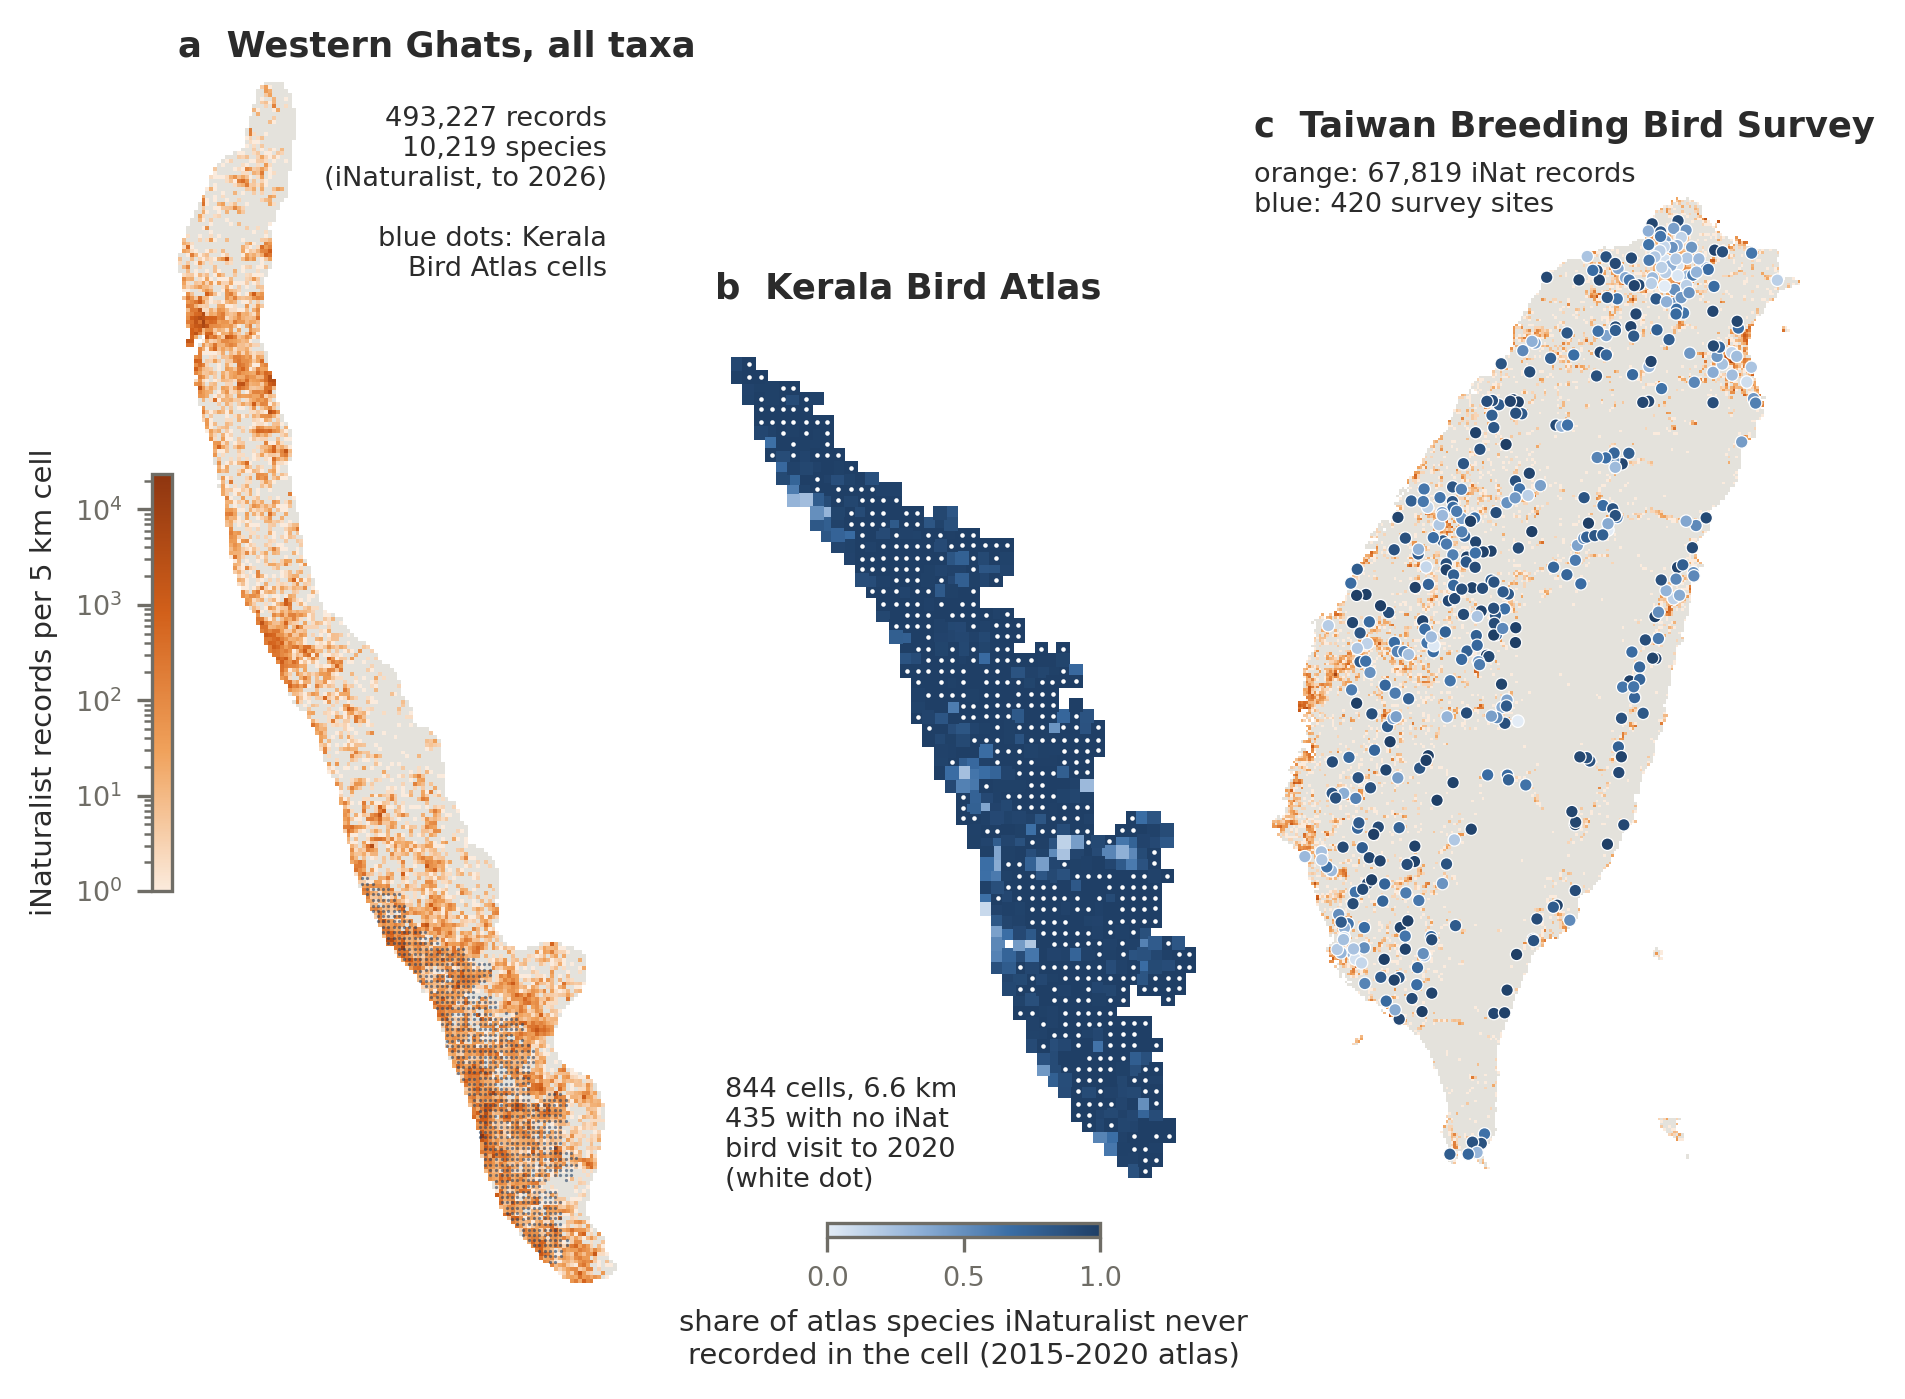
\includegraphics[width=\textwidth]{F1_study_systems.png}
\caption{The real-world data. \textbf{(a)} iNaturalist records per 5 km cell in the Western Ghats study region (log scale); dark blue dots mark the Kerala Bird Atlas cells. Record density follows the coast, the cities and the hill stations. \textbf{(b)} The 844 atlas cells, coloured by the share of atlas species that iNaturalist never recorded in the cell up to 2020. White dots mark the cells with no iNaturalist bird visit at all. \textbf{(c)} Taiwan: iNaturalist bird records per 1 km pixel up to 2022 (orange), and the 420 Breeding Bird Survey sites used as truth, coloured by the share of their survey species iNaturalist never recorded there.}
\label{fig:systems}
\end{figure}

\begin{table}[htbp]
\centering\small
\caption{Test beds. PO: presence-only records used for training. Truth: the independent data used for scoring.}
\label{tab:data}
\begin{tabularx}{\textwidth}{@{}p{2.8cm} X X p{1.7cm}@{}}
\toprule
Test bed & Training data & Truth & Used in \\
\midrule
T1 Virtual species & 30 simulated species on real Western Ghats covariates, 300 records each, sampled through the fitted observer-effort surface at three bias strengths & Known by construction & E03 \\
T2 disdat \citep{elith2020} & 52,605 PO records, 226 species, 6 regions (Australia, Canada, New Zealand, South America, Switzerland) & 53,044 presence--absence survey sites & E02 \\
T3 Western Ghats & 493,227 research-grade iNaturalist records, 10,219 species, 1 km grid (180,299 cells) & Later records (2019--2026) & E01, E04, E05 \\
T4 Kerala Bird Atlas \citep{kbadata} & iNaturalist birds, 26,226 records in 3,677 1 km pixels to 2020 & 844 atlas cells (6.6 km), up to 32 timed 15-min lists each, 2015--2020 & E09b--E16 \\
T5 Taiwan BBS \citep{twbbs} & 67,819 iNaturalist bird records to 2022 (name-matched, on land) & 420 survey sites, about 77 point counts each, 2017--2022 & E15--E17 \\
\bottomrule
\end{tabularx}
\end{table}

\paragraph{Western Ghats.} The study region is the five RESOLVE ecoregions that form the Western Ghats and the Malabar coast, buffered by 10 km: 181,347 km\textsuperscript{2} from 8\textdegree{}N to 22\textdegree{}N, gridded at 1 km in UTM zone 43N. Occurrences come from the iNaturalist open-data export \citep{inat}. We kept research-grade records identified to species with coordinate uncertainty of at most 5 km, removed institution and centroid hotspots following CoordinateCleaner \citep{zizka2019}, and clipped to the region. This left 493,227 records of 10,219 species (butterflies and moths 146,585; birds 130,317; plants 79,142; odonates 43,410; reptiles 17,084; mammals 8,670; amphibians 8,100).

\paragraph{Covariates.} Each 1 km cell carries 29 habitat layers and 5 access layers. Habitat: the 19 WorldClim 2.1 bioclimatic variables and elevation \citep{worldclim}, and the fractions of nine ESA WorldCover 2021 classes aggregated from 10 m pixels \citep{worldcover}. Access: distance to any road, to a major road, to a town, and to a protected area from OpenStreetMap \citep{osm}, plus log population density from WorldPop 2020 \citep{worldpop}. A sixth access layer, distance to a city, and distance to a river are used only in the bias measurement (E01).

\paragraph{Kerala Bird Atlas.} The atlas \citep{kbadata} surveyed every cell of a 6.6 km grid over Kerala with timed 15-minute complete checklists, run by trained volunteers in fixed wet- and dry-season rounds between 2015 and 2020. Of its cells, 844 fall inside our region with enough land pixels; the median cell has 32 lists. We harmonised atlas and iNaturalist names through the atlas's own name table. The analysed species are the 207 birds recorded by iNaturalist in at least 20 pixels (196 have enough unrecorded pairs to score).

\paragraph{Taiwan Breeding Bird Survey.} The survey \citep{twbbs} counts birds at about eight 100 m points per site, twice per breeding season, with six-minute counts. We use 2017--2022 as the truth window and keep the 420 sites surveyed in at least two of those years; a species is present at a site if it was detected there in that window. The truth unit is the set of 1 km pixels within 2 km of a site's points. iNaturalist bird records for Taiwan (218,610 in total; 67,819 on land up to 2022 after name matching) were cut from the same export. Survey and iNaturalist names were mapped to the GBIF backbone; 278 of 346 survey species match, and the 156 with at least 20 training pixels are analysed. Covariates are the same layers as in India, except that population is replaced by a smoothed built-up fraction because WorldPop has no Taiwan layer. We call a species ``Taiwan-concentrated'' if at least 90\% of its global iNaturalist records fall in Taiwan; 31 species qualify, close to the island's endemic list, and 17 are analysed.

\paragraph{disdat and virtual species.} The disdat benchmark \citep{elith2020} is the data behind \citet{elith2006} and \citet{phillips2009}: biased presence-only records paired with independent presence--absence surveys. The 30 virtual species have Gaussian niches on climate, elevation and natural land cover (prevalence 5--35\%) over the real Western Ghats grid. Their 300 records each are drawn through the observer-effort surface we fitted in E01, raised to a bias strength of 0 (none), 1 (as biased as real iNaturalist) or 2 (exaggerated).

\section{Methods}
\label{sec:methods}

\subsection{Measuring the bias (E01)}
We measured bias three ways. (i) Record intensity by distance to road: the share of records divided by the share of land in each distance band, which adds the land-area null that the widely quoted ``within 2.5 km of a road'' statistic lacks \citep{hughes2021}. (ii) Sampling effectiveness through time: new species-by-10 km cell combinations per 1,000 records, by year \citep{oliver2021}. (iii) A Python port of sampbias \citep{zizka2021}, in which records per 5 km cell are Poisson with rate $\lambda = q \exp(-\sum_j w_j d_j)$ over distances $d_j$ to roads, towns, cities, rivers and protected areas, fitted per taxon. We checked the port against the R package's MCMC on the same grid: all six Python estimates fall inside the package's 95\% credible intervals.

\subsection{Models and corrections}
\paragraph{Single-species models.} We used a capacity ladder: a GLM with quadratic terms, MaxEnt \citep{phillips2006}, boosted regression trees \citep[BRT, LightGBM;][]{friedman2001,ke2017}, a down-sampled random forest \citep{breiman2001,valavi2022}, a multilayer perceptron (MLP) and a patch CNN that sees a 9$\times$9 km window of the covariate stack \citep{deneu2021}. Each presence-only model contrasts the pixels where a species was recorded (label 1) with background pixels (label 0).

\paragraph{Corrections.} \emph{Naive}: 20,000 background pixels drawn uniformly over land. \emph{Target-group background} (TGB): the background is every pixel where any species of the same group was recorded, so presences and background share the observer process \citep{phillips2009}. \emph{Bias-covariate conditioning}: access layers are model inputs during training and are fixed at their median when predicting. \emph{Geographic thinning}: one record per species per 5 km cell.

\paragraph{Multi-species neural losses (E11, E12).} One 3-layer MLP predicts all species from the 29 habitat layers, trained as a 5-seed ensemble. We compared the assume-negative losses of SINR \citep{cole2023} (random-location negatives, same-location other-species negatives, and their mixture), a DeepMaxent-style normalised Poisson loss \citep{ryckewaert2025} with random or target-group background, and an effort-aware occupancy--detection likelihood. In the last, a pixel $i$ visited $U_i$ times (observer-days) records species $s$ with probability
\begin{equation}
P(y_{is}=1) = \psi_{is}\,\bigl[1-(1-p_{is})^{U_i}\bigr],
\label{eq:occeffort}
\end{equation}
where $\psi_{is}$ is occupancy from the shared network and $p_{is}$ is per-visit detection from a small head. A pixel never visited contributes nothing, and a pixel visited once and not recorded is weak evidence of absence. The loss is binary cross-entropy over the sampled pixels.

\subsection{Evaluation regimes}
\label{sec:eval}
The core of the study is comparing how different tests judge the same models (Fig.~\ref{fig:design}).
\begin{enumerate}\setlength\itemsep{1pt}
\item \textbf{Random 5-fold CV}: held-out presences against held-out background, the common default.
\item \textbf{Spatial-block CV}: folds of contiguous blocks sized by the covariate variogram \citep{valavi2019,ploton2020}; we repeated it at 0.5, 1 and 2 times the blockCV ranges.
\item \textbf{Later citizen-science records}: train on records up to year $T$ and score whether the species was later recorded in the cell.
\item \textbf{Independent truth}: the virtual-species surface (T1), disdat surveys (T2), the Kerala Bird Atlas (T4) or the Taiwan survey (T5).
\end{enumerate}

\paragraph{Missing-pair protocol (E09b, E17).} Let $Y_{cs}\in\{0,1\}$ be survey truth for cell $c$ and species $s$, and $R_{cs}\in\{0,1\}$ whether citizen science recorded $s$ in $c$ during training. A model's pixel predictions are averaged to cells. For each species we compute the \auc{} of the predictions against $Y_{cs}$ over the pairs with $R_{cs}=0$ only, and keep species with at least 5 presences and 5 absences among those pairs. The score answers one question: among the places citizen science never recorded this species, does the model rank the places where it actually occurs above the places where it does not? We also report the share of survey presences among each method's top-ranked 10\% of unrecorded pairs, pooled over species.

\paragraph{Same-pair truth-source test (E15).} We trained on records up to $T$ (2014 or 2017 in Kerala, 2016 or 2018 in Taiwan) and restricted scoring to pairs unrecorded up to $T$ in cells that iNaturalist visited again after $T$. Each pair then has two labels: the survey's, and whether iNaturalist later recorded the species there. Both truths judge identical pairs, so any difference in verdict comes from the truth source, not from the sample.

\begin{figure}[htbp]
\centering
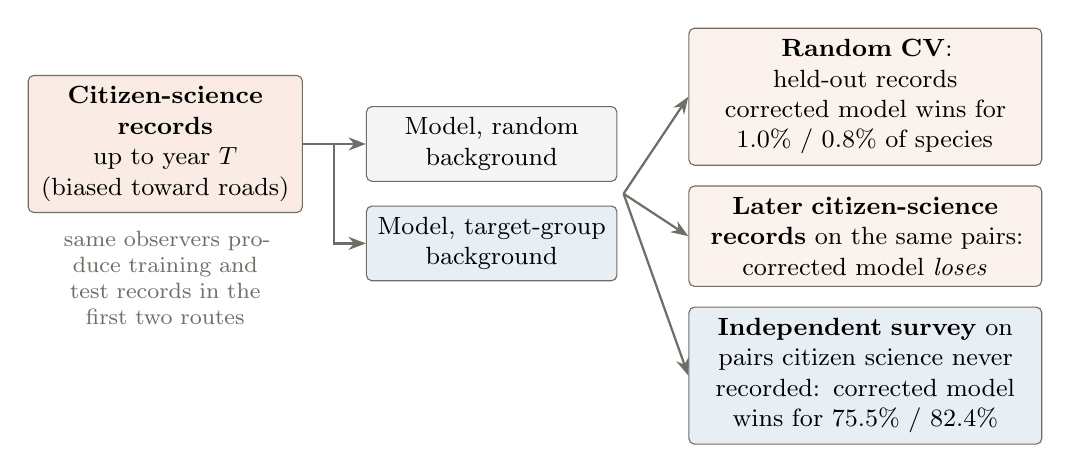
\begin{tikzpicture}[font=\small, node distance=4mm and 6mm,
  box/.style={draw=cmuted, rounded corners=2pt, align=center, inner sep=4pt, text width=#1},
  box/.default=3.1cm,
  arr/.style={-{Stealth[length=2.2mm]}, thick, cmuted}]
\node[box=3.2cm, fill=corange!12] (po) {\textbf{Citizen-science records}\\ up to year $T$\\ (biased toward roads)};
\node[box=2.9cm, right=8mm of po, fill=gray!8] (naive) {Model, random background};
\node[box=2.9cm, below=3mm of naive, fill=cblue!12] (tgb) {Model, target-group background};
\draw[arr] (po.east) -- ++(4mm,0) |- (naive.west);
\draw[arr] (po.east) -- ++(4mm,0) |- (tgb.west);
\node[box=4.2cm, right=9mm of naive, yshift=6mm, fill=corange!8] (cv) {\textbf{Random CV}: held-out records\\ corrected model wins for \KcvPick\% / \TcvPick\% of species};
\node[box=4.2cm, below=2.5mm of cv, fill=corange!8] (later) {\textbf{Later citizen-science records} on the same pairs: corrected model \emph{loses}};
\node[box=4.2cm, below=2.5mm of later, fill=cblue!12] (survey) {\textbf{Independent survey} on pairs citizen science never recorded: corrected model wins for \KtrPick\% / \TtrPick\%};
\node[fit=(naive)(tgb), inner sep=2pt] (models) {};
\draw[arr] (models.east) -- (cv.west);
\draw[arr] (models.east) -- (later.west);
\draw[arr] (models.east) -- (survey.west);
\node[below=1mm of po, text width=3.2cm, align=center, font=\footnotesize, text=cmuted] {same observers produce training and test records in the first two routes};
\end{tikzpicture}
\caption{Study design. The same pair of models (with and without the bias correction) is judged by three tests. The first two use held-out citizen-science records, which share the observer bias of the training data; the third uses an independent systematic survey. Percentages: Kerala / Taiwan.}
\label{fig:design}
\end{figure}

\paragraph{Imperfect detection in the truth (S0: E16, E17b).} An atlas ``absence'' may be a missed presence. We fitted a single-season occupancy model \citep{mackenzie2002} per species and season, with lists (Kerala) or point counts (Taiwan) as replicates. Occupancy $\psi$ depends on five principal components of the habitat layers, and detection $p$ on log observer count and time of day. For a pair with no detection in $K$ replicates, the probability that the species was present but missed is
\begin{equation}
P(\text{false absence}) = \frac{\psi\,(1-p)^{K}}{\psi\,(1-p)^{K} + 1 - \psi},
\label{eq:pfa}
\end{equation}
combined across seasons. We re-scored every headline contrast after dropping pairs whose false-absence probability exceeds 0.1, with soft labels, and with wet-only or dry-only truth. Before using the fit, we simulated detection histories with known $\psi$ and $p$ on the real list structure and checked recovery.

\subsection{Discovery forecasting (E05)}
For each 5 km cell $c$, we model the species pool as Poisson with mean $\Lambda_c$, and per-visit detection of each species as $p\sim\text{Beta}(a_c,b_c)$. After $U_c$ observer-day visits the probability that a species is still undetected is $P_0(U)=B(a_c,b_c+U)/B(a_c,b_c)$, where $B$ is the beta function. Poisson thinning then gives closed forms for observed richness, $S_c\sim\text{Poisson}(\Lambda_c[1-P_0(U_c)])$, and for the number of new species found in $m$ further visits,
\begin{equation}
N^{\text{new}}_c \sim \text{Poisson}\bigl(\Lambda_c\,[P_0(U_c)-P_0(U_c+m)]\bigr).
\end{equation}
$\log\Lambda$, $\log a$ and $\log b$ are linear in eight habitat principal components, a random-Fourier spatial field and access covariates, with Gaussian priors, fitted by MAP on the GPU. The likelihood extends the beta-binomial incidence model of \citet{chiu2022} to a spatially hierarchical forecast. Each model is fitted on records up to year $T$ and scored by log score on new species-in-cell records in $T+1$ to $T+3$, given the visits that actually happened. Baselines are a negative-binomial effort regression and Shen--Chao extrapolation \citep{shen2003}.

\subsection{Statistics}
Per-species \auc{} differences are tested with paired Wilcoxon signed-rank tests across species. Because neighbouring cells are not independent, we also report 95\% confidence intervals from a spatial-block bootstrap that resamples 0.3\textdegree{} blocks of survey cells (\Kblocks{} blocks in Kerala, \Tblocks{} in Taiwan; 1,000 replicates), recomputing every species' \auc{} in each replicate. Species-level regressions use HC3 robust standard errors, with a permutation test for the endemic coefficient. Hyperparameters were fixed in advance and never tuned on survey truth.

\section{Results}

\subsection{The bias is strong and measurable (H1)}
Records in the Western Ghats cling to roads (Fig.~\ref{fig:bias}a). The land within 100 m of a road is 19\% of the region but holds 65\% of records, an intensity 3.4 times that of uniform recording; beyond 2 km the intensity falls to 0.1. The headline statistic of \citet{hughes2021}, that 99.4\% of records lie within 2.5 km of a road, says little on its own here, because 94.9\% of the land does too. Only 14.4\% of 1 km cells hold any record (1.4\% for amphibians). Recording volume rose 61-fold from 2008 to 2025 (1,442 to 88,636 records a year), while new species-by-cell combinations per 1,000 records fell by 56\% (689 to 306; Fig.~\ref{fig:bias}b,c). The sampbias decay weights differ by taxon (Table~\ref{tab:sampbias}): bird and mammal records fall off fastest with distance from any road, amphibian records follow major roads most strongly, and mammal records are the most tied to protected areas.

\begin{figure}[htbp]
\centering
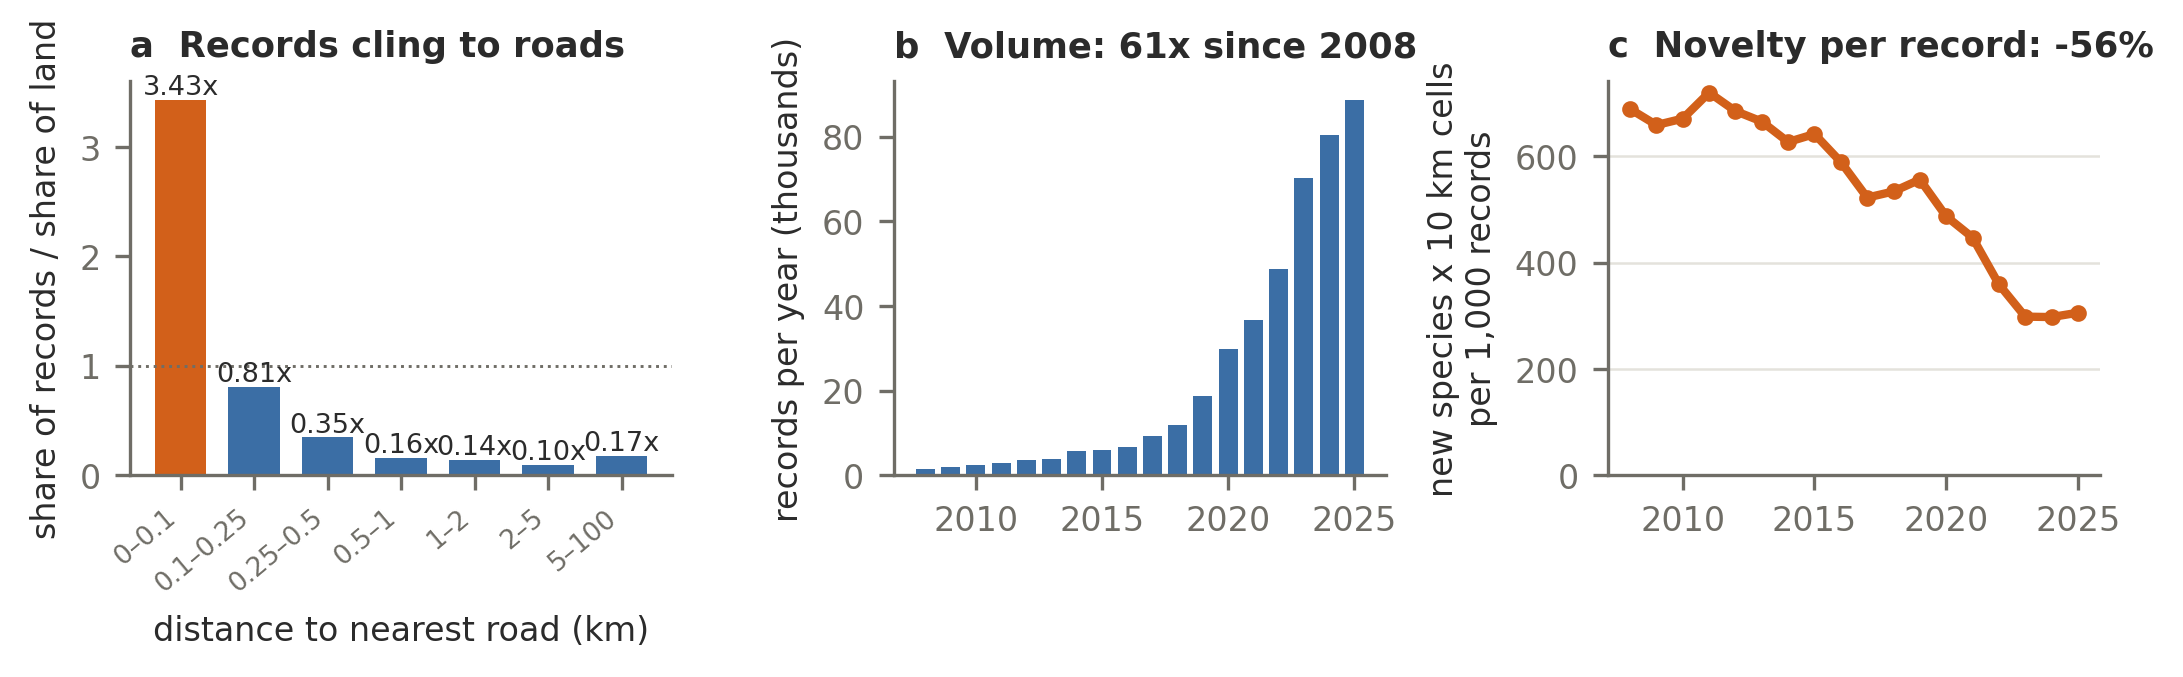
\includegraphics[width=\textwidth]{F2_bias_anatomy.png}
\caption{Bias anatomy of 493,227 Western Ghats iNaturalist records. \textbf{(a)} Recording intensity relative to land area by distance to the nearest road; 1 means recording in proportion to area. \textbf{(b)} Records per year. \textbf{(c)} Sampling effectiveness: new species $\times$ 10 km cell combinations per 1,000 records. Volume and new knowledge per record move in opposite directions.}
\label{fig:bias}
\end{figure}

\subsection{Flexible models absorb bias, and random CV rewards it (H2 to H4)}
\paragraph{Virtual species.} As bias strength rises from none to exaggerated, the true \auc{} of uncorrected models falls (mean of five models, 0.79 to 0.71), while their random-CV \auc{} rises (0.74 to 0.92; Fig.~\ref{fig:virtual}a). A better CV score is therefore evidence of more bias absorbed, not of a better map. Every flexible model leaks more of the bias into its predictions than the GLM (Fig.~\ref{fig:virtual}b; paired Wilcoxon $p\le0.003$). The most leaky model is BRT, not the CNN, so the ordering is ``flexible above linear'', not ``deeper is worse''. Of the corrections, TGB gives the highest true \auc{} at strong bias (0.757 against 0.714 uncorrected; Fig.~\ref{fig:virtual}c). It is the truly best correction for 77--90\% of species with GLM, BRT, RF and CNN, and thinning barely helps, as in \citet{inman2021}. Random CV, however, picks bias-covariate conditioning for 83--97\% of species, because that model uses accessibility directly and the biased held-out records reward it. Random CV rewards the method that models the bias best, not the one that removes it.

\begin{figure}[htbp]
\centering
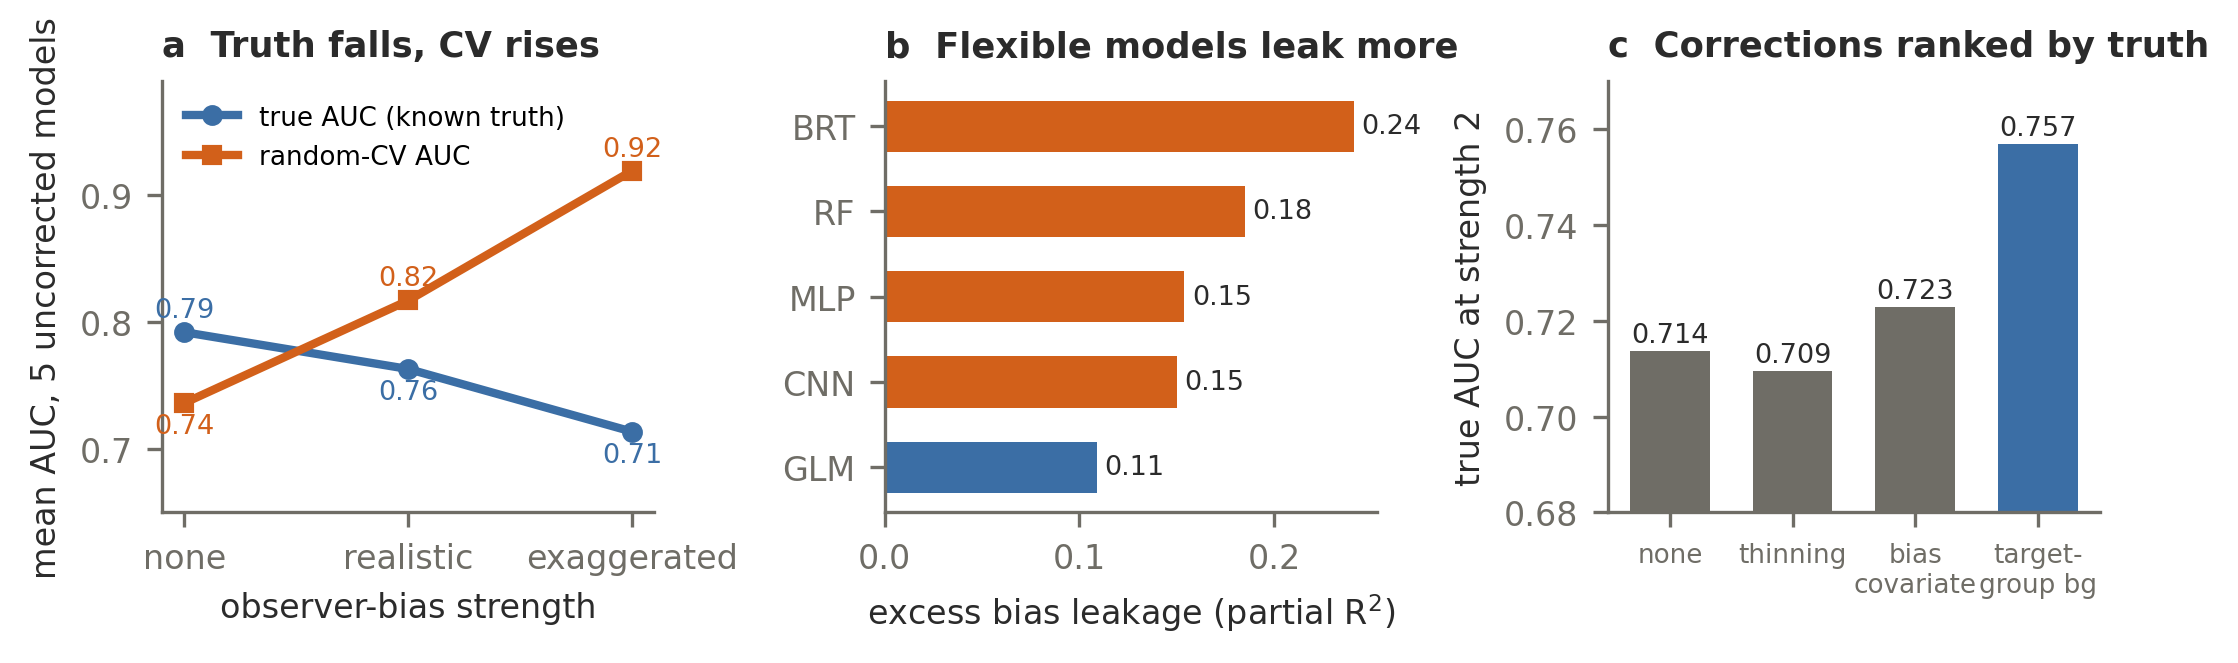
\includegraphics[width=\textwidth]{F3_virtual_species.png}
\caption{Virtual species (30 species, known truth). \textbf{(a)} Mean true \auc{} and random-CV \auc{} of five uncorrected models as observer bias strengthens. \textbf{(b)} Excess bias leakage at strength 2 (partial $R^2$ of the logit prediction on access layers beyond the true suitability, minus its value without bias). \textbf{(c)} True \auc{} of each correction at strength 2, averaged over models.}
\label{fig:virtual}
\end{figure}

\paragraph{Three real systems.} The same inversion appears on real data with independent truth (Table~\ref{tab:cv}, Fig.~\ref{fig:cv}). On disdat, the surveys prefer TGB for 62\% of the 896 species--algorithm fits (mean +0.023 \auc{}, $p=3\times10^{-16}$), reproducing \citet{phillips2009}; random CV prefers it for 4.5\%, and its verdicts are negatively rank-correlated with the truth. In Kerala and Taiwan, random CV prefers the corrected BRT for \KcvPick\% and \TcvPick\% of species, against \KtrPick\% and \TtrPick\% under survey truth. Random CV overstates the uncorrected model by \KoptNaive{} \auc{} in Kerala and \ToptNaive{} in Taiwan, but is nearly unbiased for the corrected one (\KoptTGB{} and \ToptTGB{}). Spatial blocking does not repair the verdict: larger blocks shrink the optimism of the uncorrected model (from +0.076 to +0.018 on disdat), but the share of fits on which blocked CV agrees with the truth stays at 43--44\% at every block size. Blocking removes autocorrelation optimism \citep{ploton2020}, but the held-out records still carry the observer bias. One internal check does work without survey data: scoring held-out presences against held-out \emph{target-group} sites agrees with the truth for 62\% of fits and correlates positively with it.

\begin{table}[htbp]
\centering\small
\caption{How often each evaluation says the bias correction (target-group background) helps, compared with independent survey truth. Agreement: share of fits where the evaluation and the truth agree on the sign of the difference. $\rho$: Spearman correlation between the evaluation's and the truth's \auc{} differences.}
\label{tab:cv}
\begin{tabular}{@{}llcccc@{}}
\toprule
Evaluation & $n$ & Says it helps & Truth says & Agree & $\rho$ \\
\midrule
\tabinput{tables/cv_inversion.tex}
\bottomrule
\end{tabular}
\end{table}

\begin{figure}[htbp]
\centering
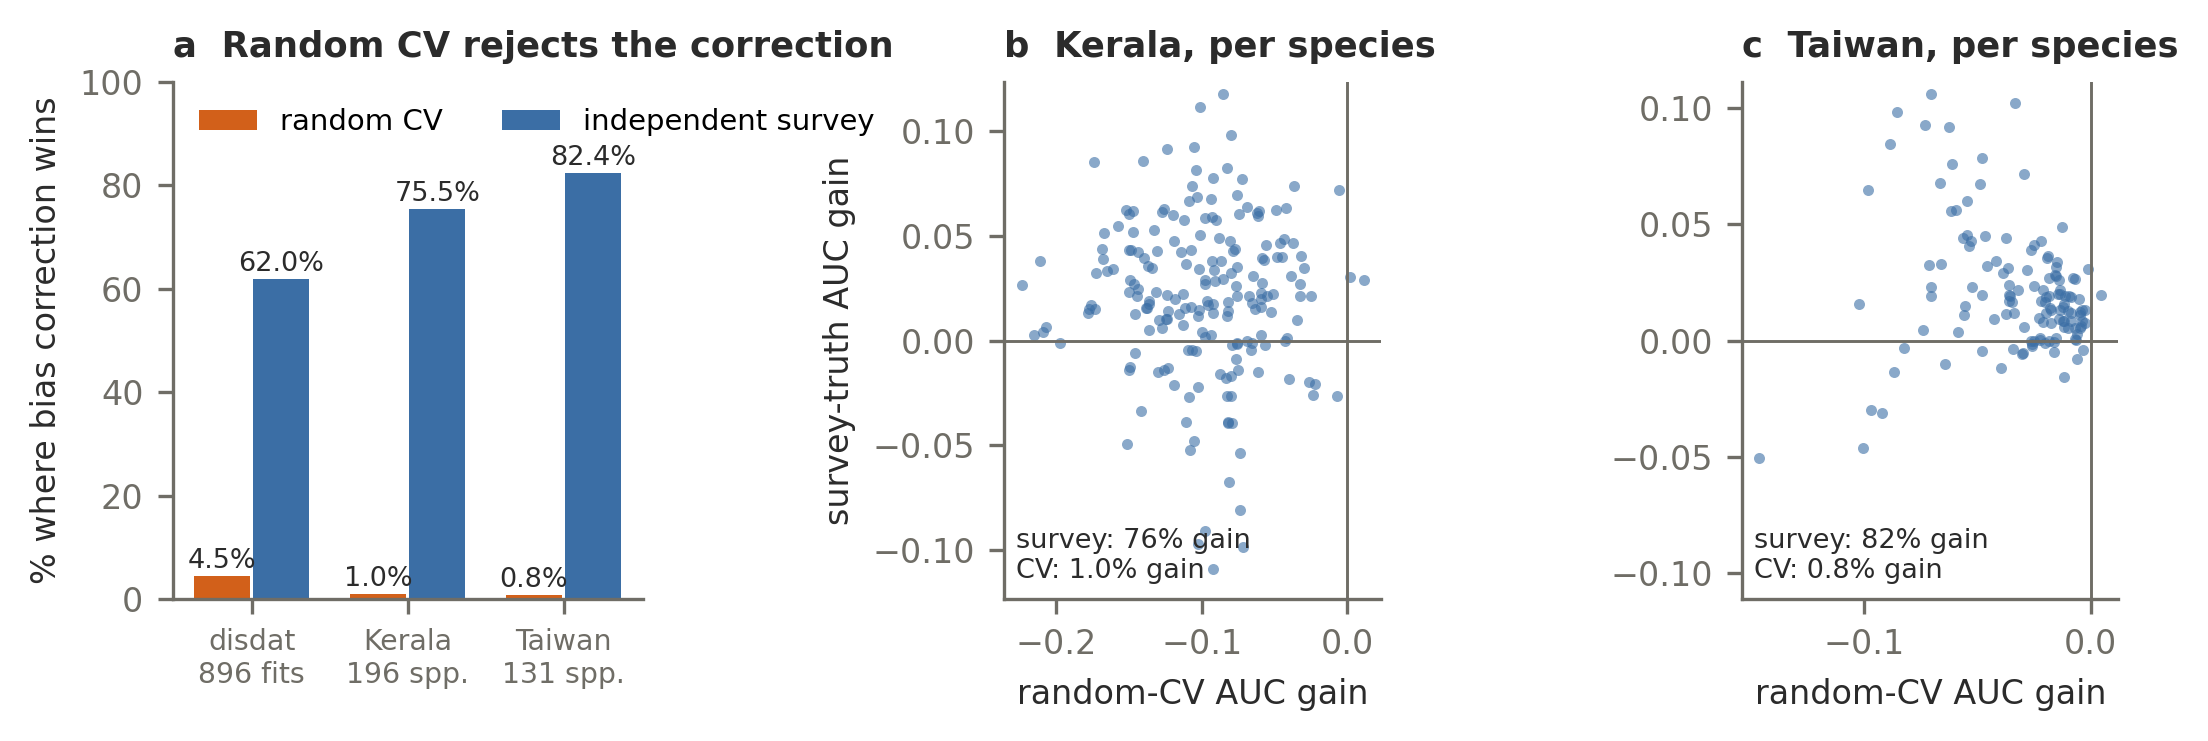
\includegraphics[width=\textwidth]{F4_cv_inversion.png}
\caption{Random cross-validation inverts the model choice. \textbf{(a)} Share of fits (disdat) or species (Kerala, Taiwan) for which random CV and independent surveys say the target-group correction improves the model. \textbf{(b, c)} Per-species \auc{} gain from the correction under random CV (x) and under survey truth (y). Almost every species falls left of zero (CV says the correction hurts) while most fall above zero (the survey says it helps).}
\label{fig:cv}
\end{figure}

\subsection{Corrected models find what citizen science missed (H5)}
The gap is large. In Kerala, 435 of the 844 atlas cells (52\%) have no iNaturalist bird record up to 2020. Even in the cells iNaturalist did visit, it recorded only 12\% of the species the atlas found there. Across the analysed species there are \KpairsN{} cell--species pairs that iNaturalist never recorded, and the atlas found the species in \Kbase\% of them. In Taiwan there are \TpairsN{} such pairs, with a survey prevalence of \Tbase\%.

Table~\ref{tab:missing} and Fig.~\ref{fig:missing} show how well each method ranks these pairs. The boosted-tree model with target-group background ranks them best or joint best in both systems: \auc{} \KaucTGB{} in Kerala and \TaucTGB{} in Taiwan. It beats the uncorrected BRT for \KpctTGB\% and \TpctTGB\% of species, and the nearest-record baseline by about 0.10 in both systems, with spatial-block confidence intervals that exclude zero. In practical terms, among the 10\% of unrecorded pairs it ranks highest, the survey finds the species \KhitTGB\% of the time in Kerala and \ThitTGB\% in Taiwan, against base rates of \Kbase\% and \Tbase\%. In Kerala, the 17 Western Ghats endemics gain most: corrected BRT scores 0.834 on them against 0.740 for nearest record, and the gain from the correction is twice as large as for widespread species (+0.040 against +0.020).

\begin{table}[htbp]
\centering\small
\caption{Ranking cell--species pairs that iNaturalist never recorded, against survey truth. \auc: mean per-species \auc{} (Kerala \KnSp{} species, Taiwan \TnSp{}). Top 10\%: share of survey presences among each method's highest-ranked 10\% of pairs, pooled over species. Brackets: 95\% spatial-block bootstrap intervals for the difference (K: Kerala, T: Taiwan).}
\label{tab:missing}
\begin{tabular}{@{}lcccc@{}}
\toprule
& \multicolumn{2}{c}{\auc} & \multicolumn{2}{c}{Top 10\% hit rate (\%)} \\
\cmidrule(lr){2-3}\cmidrule(lr){4-5}
Method & Kerala & Taiwan & Kerala & Taiwan \\
\midrule
\tabinput{tables/missing_pairs.tex}
\bottomrule
\end{tabular}
\end{table}

\begin{figure}[htbp]
\centering
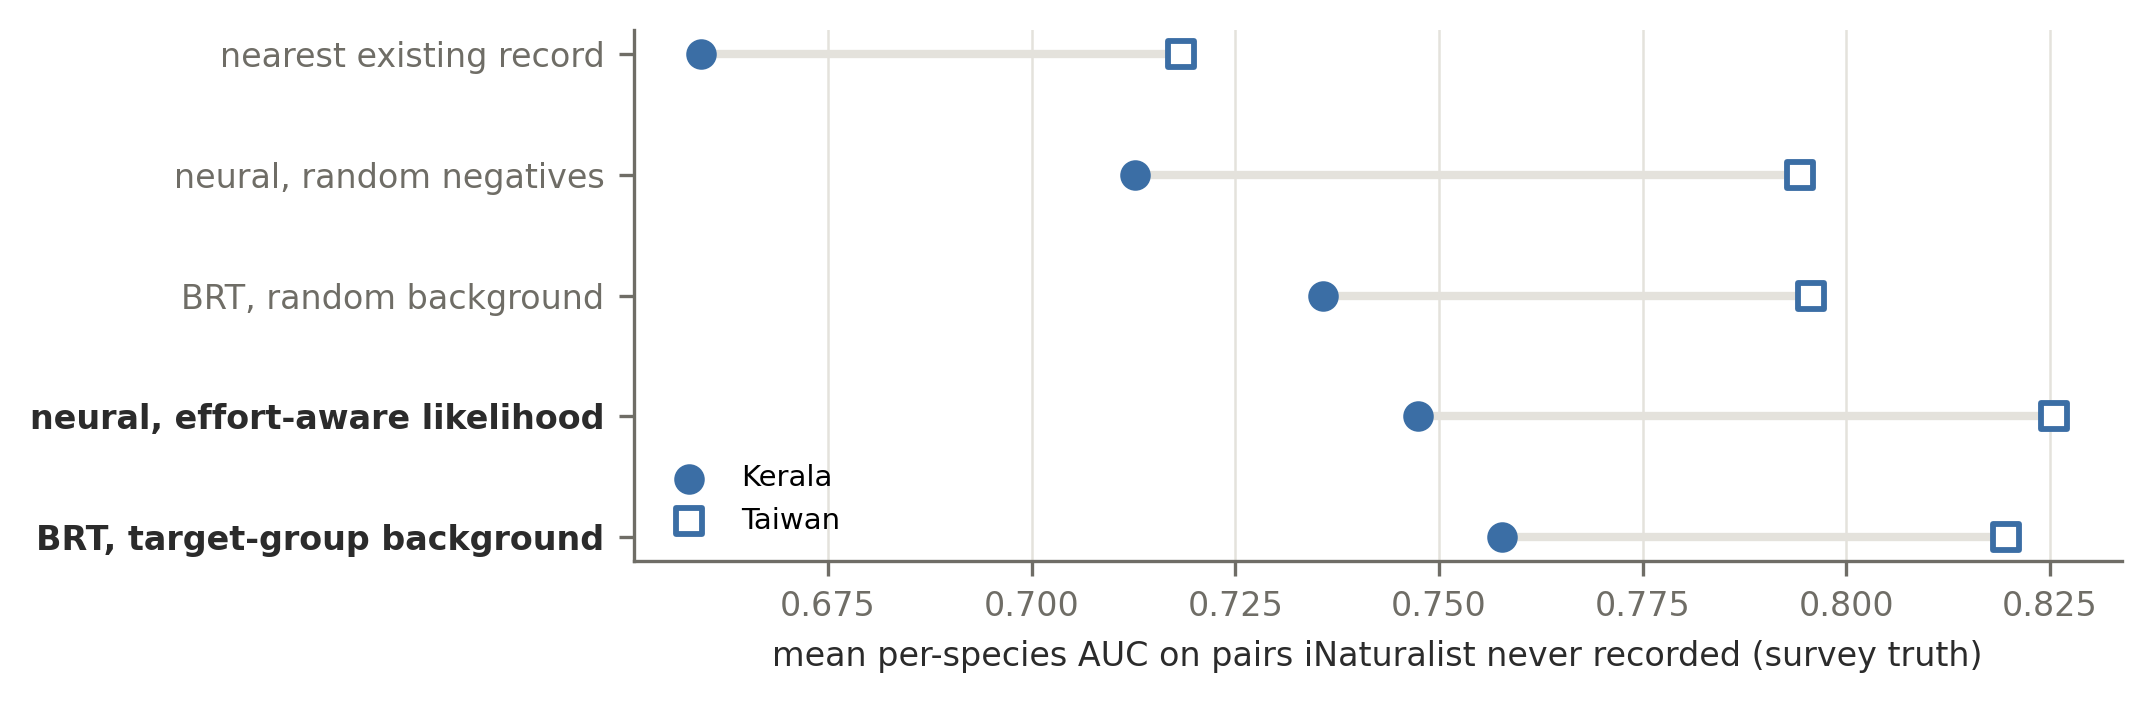
\includegraphics[width=0.88\textwidth]{F5_core.png}
\caption{Mean per-species \auc{} on the cell--species pairs iNaturalist never recorded, scored against the Kerala Bird Atlas (filled circles) and the Taiwan Breeding Bird Survey (open squares). Methods that take negatives from where people actually looked (bold) rank highest in both systems.}
\label{fig:missing}
\end{figure}

\paragraph{Neural models.} Among the neural losses (Table~\ref{tab:neural}), those that take negatives from sampled pixels beat those with random-location negatives by 0.021 to 0.035 \auc{} (69--78\% of species, $p<10^{-4}$). SINR's default mixed loss does worse than its same-location variant alone, because its random negatives bring the bias back. Our effort-aware likelihood is the best neural loss in Kerala (0.747), and its advantage over plain target-group cross-entropy is largest (+0.015) in cells with 1--5 iNaturalist visits, where treating ``not recorded'' as ``absent'' is most wrong. It does not beat BRT with TGB in Kerala ($-0.010$), so the reported advantage of DeepMaxent over BRT-TGB on disdat \citep{ryckewaert2025} does not carry over to this tropical survey. In Taiwan the effort-aware network edges ahead of BRT (\TnnDelta, 65\% of species, Wilcoxon $p=0.0006$), but the spatial-block interval includes zero (\TnnCI), so we treat the two as tied.

\begin{table}[htbp]
\centering\small
\caption{Multi-species neural losses on the Kerala unrecorded pairs (one shared MLP, 5-seed ensemble, 196 species). $\Delta$: difference from BRT with target-group background.}
\label{tab:neural}
\begin{tabular}{@{}p{6.4cm}p{3.6cm}cc@{}}
\toprule
Loss & Negatives drawn from & \auc & $\Delta$ vs BRT-TGB \\
\midrule
\tabinput{tables/neural_losses.tex}
\bottomrule
\end{tabular}
\end{table}

\subsection{Later citizen-science records reverse the verdict (H7)}
At the mid-evaluation, the topic question seemed to have a negative answer. Bias-corrected Western Ghats maps did not predict where new iNaturalist records appeared in 2019--2026. Cells flagged as gaps did yield 1.6--1.7 times more new species-by-cell records per later record, but among equally under-sampled cells that were revisited, predicted richness had no effect once later effort was controlled (negative-binomial $\beta$ = +0.005 to +0.008 per SD, 95\% CI about $\pm0.03$, for all four model and correction combinations). Correction still changed the maps: the corrected GLM moved its richest 10\% of cells out of partly built-up, heavily recorded land (7\% built, 321 records per 5 km cell) into dense forest (92\% tree cover, 127 records per cell), and cut the correlation between predicted richness and past records from 0.41 to 0.13.

The survey data explain the null. Table~\ref{tab:flip} and Fig.~\ref{fig:flip}a judge the same models on the same pairs with two truths. Against the survey, the corrected model wins in every comparison; against later iNaturalist records, it loses in every comparison. This holds at both Kerala cut-offs and both Taiwan cut-offs, for boosted trees and for the neural model. The spatial-block intervals of the two truths never overlap; in five of the six bootstrapped comparisons the later-iNaturalist interval lies entirely below zero, and in the sixth (neural model, Taiwan, training to 2016) it just includes zero. Later citizen-science records follow observers, so they reward the model that learned where observers go. Validation forward in time with citizen-science data, often recommended as the remedy for optimistic cross-validation, gives the wrong answer here.

\begin{table}[htbp]
\centering\small
\caption{The same cell--species pairs judged by two truths. $\Delta$: mean per-species \auc{} gain of the bias-corrected model (BRT: target-group minus random background; Neural: effort-aware likelihood minus random-negative loss). Brackets: 95\% spatial-block bootstrap intervals. \%: share of species improved. All Wilcoxon tests give $p<0.003$.}
\label{tab:flip}
\begin{tabular}{@{}llccccccc@{}}
\toprule
& & & \multicolumn{3}{c}{Survey truth} & \multicolumn{3}{c}{Later iNaturalist truth} \\
\cmidrule(lr){4-6}\cmidrule(lr){7-9}
Training data & Model & $n$ & $\Delta$ & 95\% CI & \% & $\Delta$ & 95\% CI & \% \\
\midrule
\tabinput{tables/flip.tex}
\bottomrule
\end{tabular}
\end{table}

\begin{figure}[htbp]
\centering
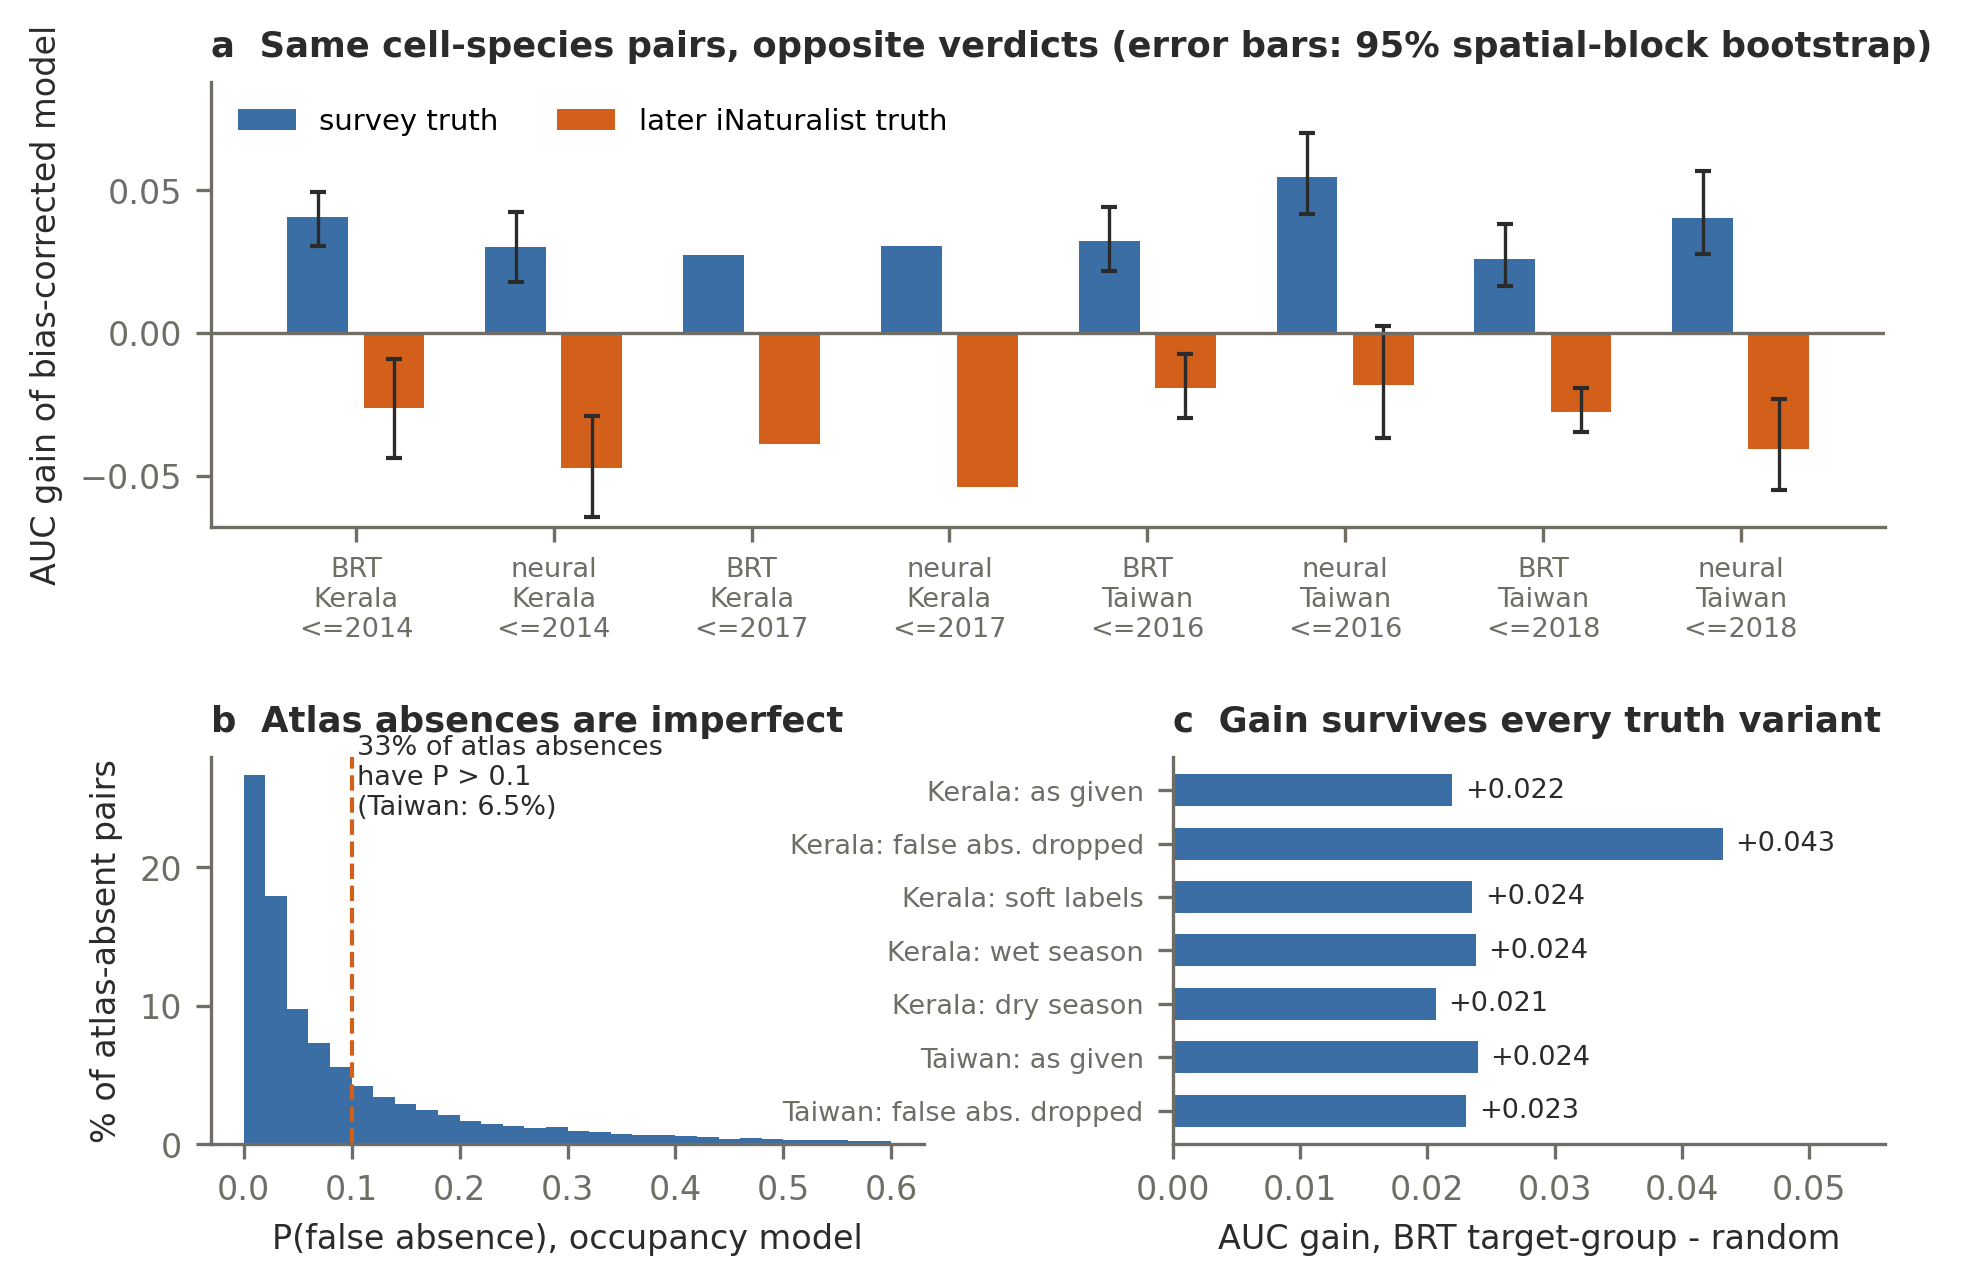
\includegraphics[width=\textwidth]{F6_flip_occupancy.png}
\caption{\textbf{(a)} The truth source decides the verdict. On identical pairs, independent surveys reward the bias-corrected model (blue) and later citizen-science records penalise it (orange). Error bars: 95\% spatial-block bootstrap (not computed for Kerala $\le$2017). \textbf{(b)} Probability that an atlas absence is a missed presence, from the occupancy model (Eq.~\ref{eq:pfa}). \textbf{(c)} The gain from target-group background under each truth variant.}
\label{fig:flip}
\end{figure}

\subsection{The survey truth is imperfect, and correcting it strengthens the result (S0)}
The atlas is a noisier truth than we had assumed. The occupancy model passed its recovery check (median error in $\psi$ 0.011, 90th percentile 0.033; predicted false-absence rate 0.071 against a true 0.073). Median per-list detection is only 0.08, the mean probability that an atlas absence is a missed presence is 0.12, and a third of atlas-absent pairs exceed 0.1 (Fig.~\ref{fig:flip}b). The Taiwan survey, with about 77 point counts per site, is cleaner: the mean is 0.023 and 6.5\% exceed 0.1.

Every result survives, and the Kerala ones get stronger (Fig.~\ref{fig:flip}c). Dropping likely false absences raises the BRT gain from +0.022 to +0.043, the neural gain from +0.035 to +0.071, and the same-pair survey gain from +0.040 to +0.060. Model rankings are identical under all five truth variants, including wet-season against dry-season truth (Kendall $\tau=1$). The missed presences sit where species are likely to occur, so treating the atlas as perfect penalised good models: our headline gains were understated.

A side result concerns detection. Across species, the per-visit ``detection'' that the effort-aware network learns from iNaturalist is negatively correlated with the atlas's real per-list detection (Spearman $-0.54$). Species that atlas surveyors detect easily, the common and vocal birds, get \emph{low} iNaturalist detection. The parameter measures what iNaturalist users choose to photograph and upload, not how detectable a bird is. Detection parameters fitted to opportunistic data should not be read as detectability.

\subsection{Which species gain? (H8)}
In Kerala, the extra gain for endemics disappears once we account for \emph{exposure}, the share of a species' atlas cells that iNaturalist never visited (Fig.~\ref{fig:endemic}a). The endemic coefficient falls from +0.020 ($p=0.005$) to +0.005 ($p=0.52$) when exposure enters the model, and exposure itself is strongly positive (+0.263, $p<10^{-4}$). Endemics are simply more exposed (0.53 against 0.47). This fits the theory of \citet{botella2020}: target-group background helps species whose ranges are anti-correlated with sampling effort. It also reconciles our result with \citet{ranc2017}, who found that correction can hurt narrow-ranging virtual species: what matters is how a range lines up with effort, not range size.

Taiwan does not replicate this mechanism (Fig.~\ref{fig:endemic}c). Taiwan-concentrated species also gain more (+0.033 with covariates, $p=0.0002$, permutation $p=0.0005$), yet they are \emph{less} exposed to unvisited cells than other species (0.34 against 0.47). What does replicate is elevation (Fig.~\ref{fig:endemic}b,d). Species with higher-elevation ranges gain more in both systems: +0.031 per km in Kerala, and +0.031 (training to 2016) and +0.022 (to 2018) per km in Taiwan, in models that also include exposure, training size and prevalence. Our reading is that montane assemblages are where a random-background model most often confuses ``rarely visited'' with ``unsuitable''. The Kerala exposure mechanism should be read as system-specific.

\begin{figure}[htbp]
\centering
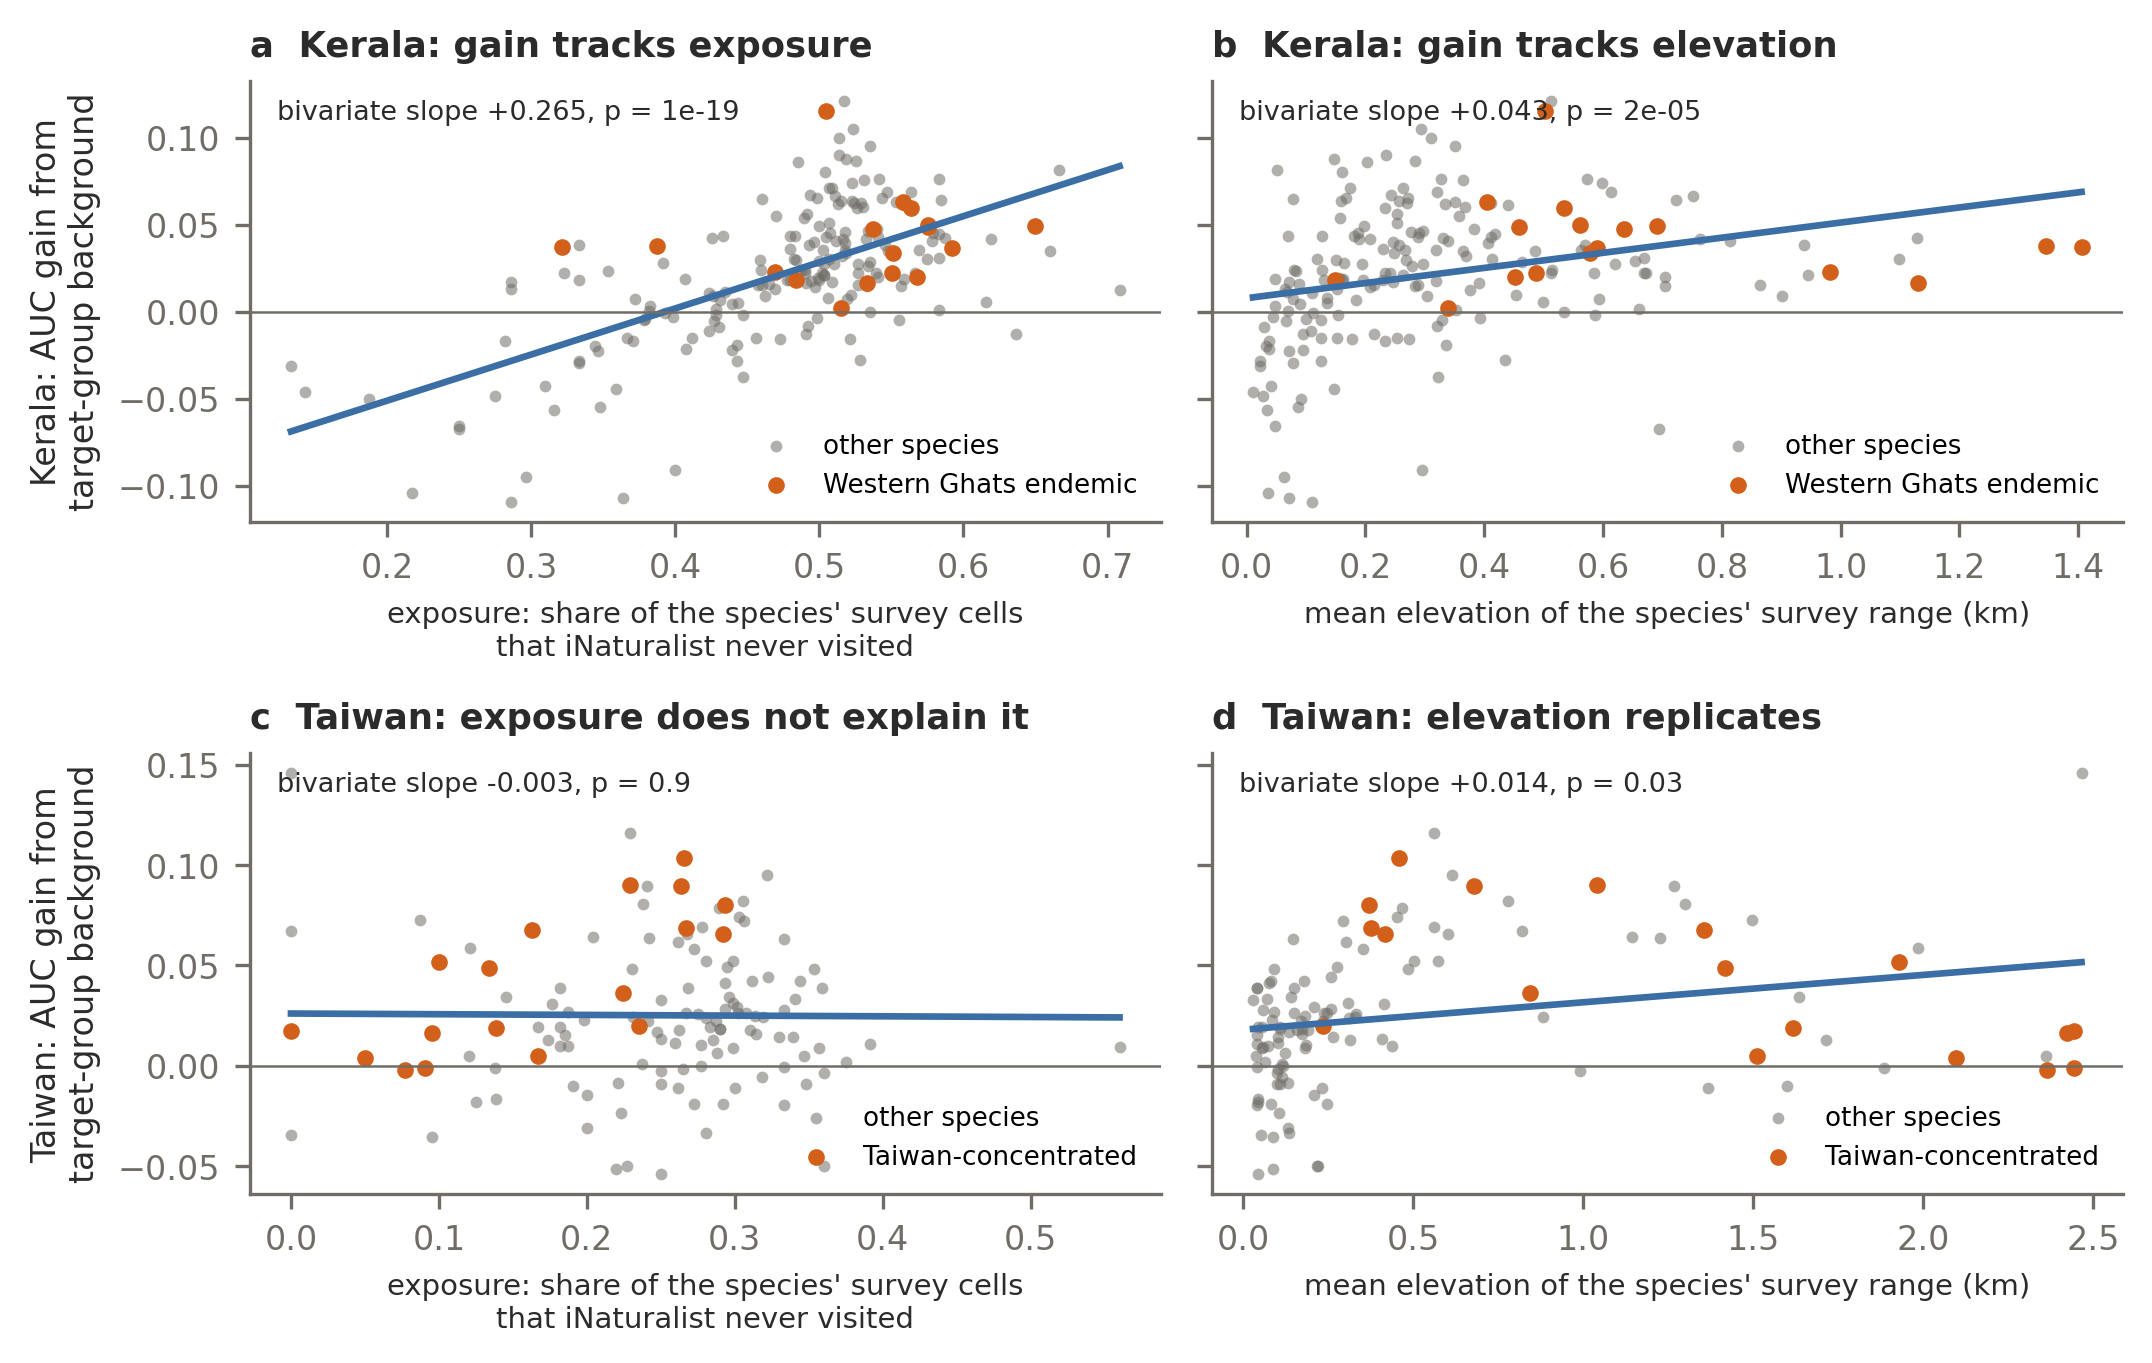
\includegraphics[width=\textwidth]{F7_endemic_elevation.png}
\caption{Which species gain from target-group background. Each point is a species; orange marks Western Ghats endemics (Kerala) or Taiwan-concentrated species. Lines are bivariate OLS fits (HC3 $p$-values); the coefficients quoted in the text come from multiple regressions. Taiwan panels use the 2018 training cut-off.}
\label{fig:endemic}
\end{figure}

\subsection{A Bayesian model of sampling forecasts discovery (H6)}
The richness maps did not predict new citizen-science records, but a model of the sampling process did (Fig.~\ref{fig:discovery}a). The beta-binomial discovery model beats the effort regression at every forecast origin: +0.022, +0.054, +0.039 and +0.020 nats per 5 km cell for origins 2016 to 2022, with spatial-block intervals that exclude zero (2016 only just). Adding the same habitat covariates to an ordinary regression makes it worse, and Shen--Chao extrapolation fails badly ($-4$ to $-5$ nats), because it cannot forecast unsampled cells. An ablation shows that the gain comes from the detection-and-saturation structure: the intercepts-only model does as well as the full one. Habitat covariates do help the model \emph{rank} cells by discovery rate (Spearman 0.22--0.36 against the realised rate). By taxon (Table~\ref{tab:taxa}), odonates, birds, butterflies and reptiles gain significantly; plants do not.

\begin{figure}[htbp]
\centering
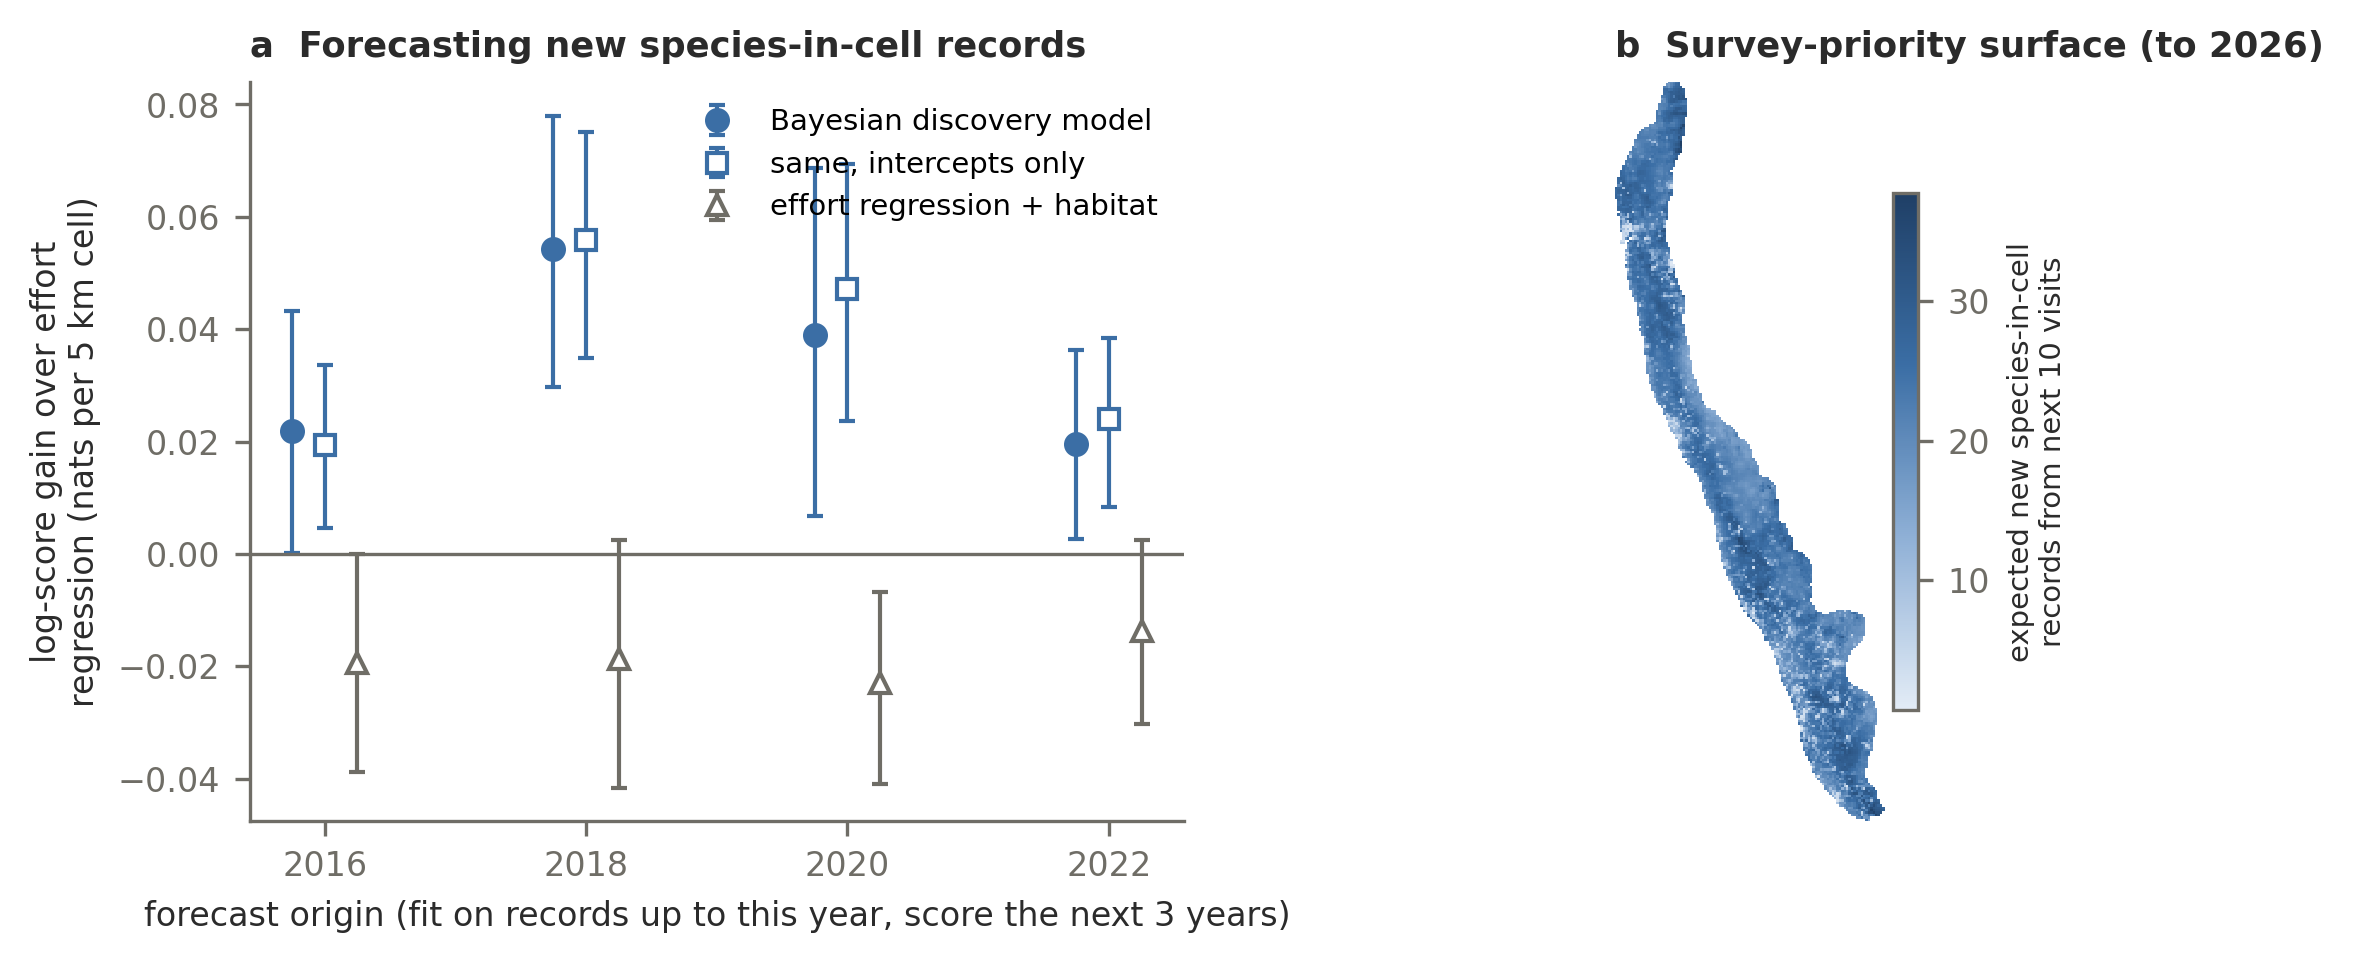
\includegraphics[width=\textwidth]{F8_discovery.png}
\caption{\textbf{(a)} Log-score gain in forecasting new species-in-cell records over the next three years, relative to a negative-binomial effort regression (95\% intervals from 50 km block bootstrap). Shen--Chao extrapolation scores between $-5.3$ and $-4.0$ (off scale). \textbf{(b)} Expected new species-in-cell records from the next 10 visits to each 5 km cell, fitted on all records to 2026.}
\label{fig:discovery}
\end{figure}

The model has two clear limits. On GeoLifeCLEF Europe \citep{glc2024}, where presence-only records carry no observer identity and a ``visit'' had to be defined as publisher $\times$ day, it loses to the regression at every origin ($-0.13$ to $-0.19$ nats per cell): one publisher-day can hold thousands of records, detection per visit becomes nearly certain, and the saturation curve collapses. The model's edge depends on a meaningful unit of effort. And its probability of a species remaining undetected ranks the Kerala atlas cells by fraction missed no better than ``fewest visits'' (Spearman 0.832 against 0.847), while classical Chao2 points the wrong way ($-0.84$). It forecasts how many new records the next visits will add; it does not estimate true missing richness.

\section{Discussion}

\paragraph{The answer to the topic question.} Environmentally predicted patterns do reveal biodiversity that citizen science misses, but only when both the model and its test account for observer bias. Against two independent bird surveys, a boosted-tree model with target-group background ranks the species citizen science never recorded in a cell at \auc{} 0.76--0.82, and roughly doubles the hit rate of a field visit chosen at random among unrecorded pairs (\KhitTGB\% against \Kbase\% in Kerala, \ThitTGB\% against \Tbase\% in Taiwan). The correction is what makes the model better than an uncorrected one. The useful outputs are maps of where specific species are likely to have been missed, not a single richness map, and a forecast of how many new records further visits will produce.

\paragraph{Why biased tests reward biased models.} Random CV, spatially blocked CV and forward validation against later citizen-science records all hold out records produced by the same observers as the training data. A model that has learned where observers go is therefore rewarded by all three. The virtual species show the mechanism directly: CV \auc{} rises while true \auc{} falls as bias grows. The real data show its consequence: CV prefers the uncorrected model for about 99\% of species in both bird systems, and later records reverse the survey's verdict on identical pairs. Earlier work established from simulation that internal evaluation is unreliable for judging bias corrections \citep{elgabbas2018,baker2024}. Our contribution is a real-data demonstration on identical pairs, in two systems, with effect sizes. Its practical implication is that a forward-in-time test with citizen-science data cannot validate a bias correction, and that independent survey data, even a modest amount, are worth more than any internal check. Where no survey exists, scoring held-out presences against held-out target-group sites was the only internal check that agreed with the truth more often than not.

\paragraph{Why target-group background works.} Target-group background does not try to remove accessibility from the covariates. It changes \emph{which places a presence is compared against}, so that both sides of the contrast share the observer process and the model has nothing to gain from learning where people go. The neural results point the same way: every loss that took its negatives from sampled pixels beat every loss that took them from random land, and the effort-aware likelihood of Eq.~\ref{eq:occeffort}, which changes the comparison through the number of visits, was the best neural loss. Corrections that act on the comparison set or the likelihood were the reliable ones throughout.

\paragraph{Limitations.} The independent truth covers birds only, and the Indian truth covers Kerala only; the northern Western Ghats have no systematic survey in our data. eBird data, which hold most Indian bird records, were not accessible to us, and the US Breeding Bird Survey download is behind a bot check that we did not try to bypass, so the second system is Taiwan. The Taiwan truth unit is a 2 km neighbourhood of survey points rather than a grid cell, and its population layer is a built-up proxy. Atlas truth itself misses nocturnal and secretive species; the occupancy model addresses imperfect detection but not species the survey cannot detect at all. iNaturalist obscures coordinates for threatened species, which affects Western Ghats amphibians and reptiles most. The discovery model needs observer identity to define a visit, and on GeoLifeCLEF, which lacks it, the model loses to the regression. Finally, the novelty claims rest on targeted literature searches.

\paragraph{Recommendations.} (1) Use target-group background, or a likelihood that takes negatives from where people looked, as the default correction. (2) Do not validate a bias correction with random CV, blocked CV or later citizen-science records; obtain independent survey data, and when none exist, test against held-out target-group sites. (3) Score models on the pairs citizen science never recorded, since that is where gap-filling claims are made. (4) Model imperfect detection in the truth data before trusting absences. (5) Keep observer identity with citizen-science records, because it is what makes discovery forecasting possible.

\section{Conclusion}
Bias-corrected species distribution models can find birds that citizen science never recorded, in two independent systems, and endemic and montane species benefit most. The evidence for this is invisible to the evaluations most often used. Random cross-validation prefers the uncorrected model for nearly every species, and later citizen-science records reverse the survey's verdict on the same pairs. A simple change to the background sample, drawing it from where people actually looked, was the most reliable correction, and the gains it brings grow once imperfect detection in the survey is modelled.

\section*{Data and code availability}
\sloppy
All data are open: iNaturalist via the open-data export; WorldClim, ESA WorldCover, WorldPop and OpenStreetMap; disdat via the R package; the Kerala Bird Atlas from Dryad (doi:10.5061/dryad.zpc866t8g); and the Taiwan Breeding Bird Survey via GBIF (doi:10.15468/qqkhd5). The analysis code (experiments E01 to E19) is in the project repository, and every number in this paper is regenerated by a script there.

\section*{Author contributions}
All four authors contributed to the literature review, study design, analysis and writing.

\bibliographystyle{apalike}
\bibliography{refs}

\appendix
\section{Supplementary tables}

\begin{table}[h]
\centering\small
\caption{sampbias decay weights per km of distance (larger: records fall off faster with distance), Western Ghats iNaturalist records. All Python estimates fall inside the 95\% credible intervals of the R package fitted on the same 5 km grid.}
\label{tab:sampbias}
\begin{tabular}{@{}lrcccccc@{}}
\toprule
Records & $n$ & Any road & Major road & Town & City & River & Protected area \\
\midrule
\tabinput{tables/sampbias.tex}
\bottomrule
\end{tabular}
\end{table}

\begin{table}[h]
\centering\small
\caption{Discovery model by taxon, forecast origin 2018: log-score gain over the effort regression (nats per 5 km cell) with 95\% spatial-block bootstrap intervals.}
\label{tab:taxa}
\begin{tabular}{@{}lrcc@{}}
\toprule
Group & Cells & Gain & 95\% CI \\
\midrule
\tabinput{tables/discovery_taxa.tex}
\bottomrule
\end{tabular}
\end{table}

\end{document}
